%%%%%%
%
% $Autor: Wings $
% $Datum: 2020-01-18 11:15:45Z $
% $Pfad: WuSt/Skript/Produktspezifikation/powerpoint/ImageProcessing.tex $
% $Version: 4620 $
%
%%%%%%


\section{Limits of Artificial Intelligence}

Image recognition has made huge progress in recent years \cite{}. Nevertheless, limitations are also becoming apparent. In this context, the image of a panda from a paper by Ian Goodfellow and other researchers is shown \cite{Goodfellow:2014}. An algorithm identifies the panda with a probability of 57{,}7\%. If the image is overlaid with a second image that a human perceives as noise, a gibbon is identified with a probability of 99{,}3, even though in a human's eyes the image has not changed. The situation is illustrated in Figure~\ref{Adversarial:Panda}.

\begin{figure}
    \includegraphics[page=3,width=0.9\textwidth,viewport=20 600 560 900,clip]{../../MLbib/Adversarial/1412.6572.pdf}
    
    \caption{Overlay of the image of a panda with noise
    	    \cite{Goodfellow:2014}}\label{Adversarial:Panda}
\end{figure}

The example with the Panda is harmless. In contrast, the effects in road traffic can be devastating. Research shows that by simply manipulating road signs, artificial intelligence can make false interpretations. \cite{Sitawarin:2018} Well-defined manipulations can be carried out by selectively altering an image. In the image~\ref{Adversarial:Stop}, a sign marking a speed limit is transformed into a stop sign by adding spots. 



\begin{figure}
  \centering
  \includegraphics[page=2,width=0.4\textwidth,viewport=20 450 180 600,clip]{../../MLbib/Adversarial/1802.06430.pdf}
    
  \caption{Manipulation of traffic signs  \cite{Sitawarin:2018}}\label{Adversarial:Stop}
\end{figure}

Conversely, an optimal image can be determined from the neuronal networks that delivers a result with a probability close to 100\%. This also produces images that the human eye could not recognise as such. A classic example is the toaster in the image~\ref{Adversarial:Toaster}.\cite{Brown:2017}


\begin{figure}
    \includegraphics[page=2,width=0.9\textwidth,viewport=20 470 560 900,clip]{../../MLbib/Adversarial/1712.09665.pdf}
    
    \caption{Optimal image for the identification of a toaster  \cite{Sitawarin:2018}}\label{Adversarial:Toaster}
\end{figure}

